% \pagebreak[4]
% \hspace*{1cm}
% \pagebreak[4]
% \hspace*{1cm}
% \pagebreak[4]

\chapter{Results and Discussion}
\ifpdf
    \graphicspath{{Results/ResultsFigs/PNG/}{Results/ResultsFigs/PDF/}{Results/ResultsFigs/}}
\else
    \graphicspath{{Results/ResultsFigs/EPS/}{Results/ResultsFigs/}}
\fi

\cmpd*{cmpd:bromoacid}
\cmpd*{cmpd:meoamide}
\cmpd*{cmpd:bromoamide.{one,two}}
\cmpd*{cmpd:xanthateamide.{one,two}}
\cmpd*{cmpd:thioamide.{one,two}}
\cmpd*{cmpd:DMTamide.{one,two}}
\cmpd*{cmpd:DMTaldehyde.one}
\cmpd*{cmpd:DMTaldehyde.two}

\section{Synthesis of 2-mercapto-2-phenylacetaldehyde auxiliaries}

  \begin{scheme}
      \cmpdref{cmpd:DMTaldehyde.one}
      \cmpdref{cmpd:DMTaldehyde.two}
      \includegraphics[max width=\textwidth]{twoauxiliaries.eps}
      \caption{2-mercapto-2-phenylacetaldehyde ligation auxiliaries \label{sch:TwoAuxiliaies}}
  \end{scheme}

  In the initial part of this project we synthesized a set of two S-protected 2-mercapto-2-phenylacetaldehyde auxiliaries \cmpd{cmpd:DMTaldehdye.one} and \cmpd{cmpd:DMTaldehyde.two} starting from commercially available phenylacetic acids via a 6-step route (\ref{sch:OverallScheme}). Both auxiliaries were prepared successfully with good overall yields.

  The auxiliaries were synthesised bearing an acid-labile 4,4'-dimethoxytrityl (DMT) thiol protecting group to prevent thioacetal formation. The DMT protecting group was selected as it is rapidly removed  under the acidic conditions employed to cleave the auxiliary-peptides from the SPPS support resin.

  \begin{scheme}[H]
      \cmpdref{cmpd:bromoacid}
      \cmpdref{cmpd:meoamide}
      \cmpdref{cmpd:bromoamide.{one,two}}
      \cmpdref{cmpd:xanthateamide.{one,two}}
      \cmpdref{cmpd:thioamide.{one,two}}
      \cmpdref{cmpd:DMTamide.{one,two}}
      \cmpdref{cmpd:DMTaldehyde.{one,two}}
      \includegraphics[width=0.8\textwidth]{overall-scheme.eps}
      \caption[Synthesis of the ligation auxiliaries]{Key: (a\textsubscript{1}) N-bromosuccinimide, irradiation, DCM, (\SI{71}{\percent}); (a\textsubscript{2}) N-bromosuccinimide, AIBN, DCM, (\SI{83}{\percent} crude); (b\textsubscript{1}) N,O-dimethylhydroxylamine, \ch{EDC.HCl}, \ch{Et3N}, dry DCM, (\SI{90}{\percent} crude); (b\textsubscript{2}) N,O-dimethylhydroxylamine, EDC.HCl, \ch{Et3N}, dry DCM, (\SI{90}{\percent} crude); (c) Potassium ethyl xanthate, acetone, (R=Br, \SI{85}{\percent}), (R=OMe, \SI{48}{\percent} for 2 steps); (d) piperidine, DCM, (R=Br, \SI{41}{\percent}), (R=MeO, \SI{73}{\percent}); (e) \IUPAC{4,4'-dimethoxytrityl chloride}, \ch{Et3N}, dry DCM, (R=Br, \SI{84}{\percent}), (R=OMe, \SI{79}{\percent}); (f) \ch{LiAlH4}, THF, (R=Br, \SI{60}{\percent}), (R=OMe, \SI{78}{\percent}); \label{sch:OverallScheme}}
  \end{scheme}

  The initial benzylic bromination of 4-bromophenylacetic proceeded cleanly to provide \cmpd{cmpd:bromoacid}. However attempts to synthesize 2-bromo-2-(4-methoxyphenyl)acetic acid under identical conditions failed with the formation of a complex mixture of products. Efforts to perform the radical bromination on the 4-methoxyphenylacetic acid substrate under milder conditions (NBS, AIBN, \SI{30}{\celsius}) also yielded a complex mixture of products which were not readily purifiable by flash chromatography.

  A literature review indicated that 4-methoxyphenylacetic acid can undergo rapid decarboxylation to produce a benzylic radical via an intermediate aromatic radical cation\cite{steenken_generation_1990}. To avoid this decomposition pathway, the route to \cmpd{cmpd:bromoamide.two} was modified to first form the Weinreb amide \cmpd{cmpd:meoamide} as amides cannot the undergo the undesired decarboxylation process. A subsequent AIBN promoted benzylic bromination on the amide afforded \cmpd{cmpd:bromoamide.two} which was used without further purification. The formation of a Weinreb amide before radical bromination is likely to provide the most consistent results when synthesizing future substituted 2-mercapto-2-phenylacetaldehyde auxiliaries.

  The subsequent steps to the protected auxiliaries \cmpd{cmpd:DMTaldehyde.one} and \cmpd{cmpd:DMTaldehyde.two} proceeded smoothly and both compounds were obtained as red crystalline solids in acceptable yields overall (\cmpd{cmpd:DMTaldehyde.one}=\SI{12}{\percent}, \cmpd{cmpd:DMTaldehyde.two}=\SI{18}{\percent}).

\section{Synthesis of the model peptide}

The model peptide \cmpd{cmpd:modelpeptide} with sequence \ce{H-GRAEYSGLG-NH2} was synthesised on an automated peptide synthesiser by standard Fmoc/t-Bu based SPPS on Tentagel Rink amide PEG resin. A N-terminal glycine site was selected for our initial research in order to minimize the potential for side chain interface during ligation or auxiliary removal.

\section{Introduction of ligation auxiliaries to the model peptide}

  \begin{scheme}[H]
      \cmpdref{cmpd:DMTaldehyde.{one,two}}
      \cmpdref{cmpd:auxiliarypeptide.{one,two}}
      \includegraphics[width=0.8\textwidth]{reductive-amination.eps}
      \caption{Reductive amination of auxiliary to peptide \cmpd+{cmpd:modelpeptide} on solid support.\label{sch:reductiveamination}}
  \end{scheme}

  The auxiliary aldehydes \cmpd{cmpd:DMTaldehyde.one, cmpd:DMTaldehyde.two} were coupled to the N-terminus of the resin-supported model peptide \cmpd{cmpd:modelpeptide} under unoptimized reductive amination conditions (\ref{sch:reductiveamination}). The auxiliary-peptides were subsequently cleaved from the resin (95:5 TFA/TIS; \SI{2}{\hour}), precipitated from cold ether and purified by preparative HPLC.

  % A solution of respective auxiliary and \ch{NaBH3CN} in NMP:IPA:AcOH (3:1:\SI{5}{\percent}) was shaken with the model peptide on solid support for \SI{12}{\hour}.

  The desired unprotected auxiliary peptides \cmpd{cmpd:auxiliarypeptide.{one, two}} were isolated as white powders in acceptable yields (\cmpd{cmpd:auxiliarypeptide.{one}}=\SI{7.77}{\percent}, \cmpd{cmpd:auxiliarypeptide.{two}}=\SI{24.4}{\percent}) (\ref{fig:auxpepuplc}). It may be advantageous to introduce the auxiliary to the peptide via a two step approach.  The auxiliary would initial be reductively aminated to the desired N-termni amino acid in solution.\cite{tchertchian_synthesis_2004}. The auxiliary-amino acid could then be coupled to the peptide N-terminus under proven peptide coupling conditions.

  \subsection{Peptide Ligation}

    With the desired auxiliary-peptides in hand, we began to examine their ability to facilitate peptide ligation. We selected an exemplar peptide thioester \cmpd{cmpd:thioester} (H-LYRAG-MPA-G-NH2) for all our ligations. This thioester in used as a model across many NCL studies \cite{blanco-canosa_efficient_2008} and consequently it was available within our research group.

    \begin{scheme}[!htpb]
        \cmpdref{cmpd:thioester}
        \cmpdref{cmpd:auxiliarypeptide.{one,two}}
        \cmpdref{cmpd:auxiliarydipeptide.{one,two}}
        \includegraphics[width=0.8\textwidth]{auxiliary-ligation.eps}
        \caption{Ligation of auxiliary-peptide and thioester.\label{sch:auxiliaryncl}}
    \end{scheme}

    The ligations of auxiliary-peptides \cmpd{cmpd:auxiliarypeptide.one} and \cmpd{cmpd:auxiliarypeptide.two} with the alkyl peptide-thioester \cmpd{cmpd:thioester} were carried out under standard NCL conditions (100 mM \ch{Na2HPO4}, pH 7.5, RT) in degassed phosphate ligation buffer. The reducing agent TCEP was added to the ligation buffer at 100 mM concentration to prevent disulfide bond formation. Additionally \SI{3}{\percent} thiophenol was introduced to promote the \insitu conversion of our alkyl thioester to a more reactive aryl thioester\cite{dawson_modulation_1997}. Auxiliary peptide solubility issues were mitigated by the use of denaturating aqueous guanidine as the ligation solvent.

    \subsubsection{Ligation of Auxiliary Peptide \cmpd+{cmpd:auxiliarypeptide.one}}

    UPLC analysis shows that the ligation of \cmpd{cmpd:auxiliarypeptide.one} and the model thioester occurs rapidly with almost complete consumption of the auxiliary peptide observed within \SI{30}{\minute}. A small excess of \cmpd{cmpd:auxiliarypeptide.one} was used in this ligation and as a result the excess auxiliary is observable at the \SI{150}{\minute} point in \ref{fig:brligation}.

    \begin{figure}[!htbp]
        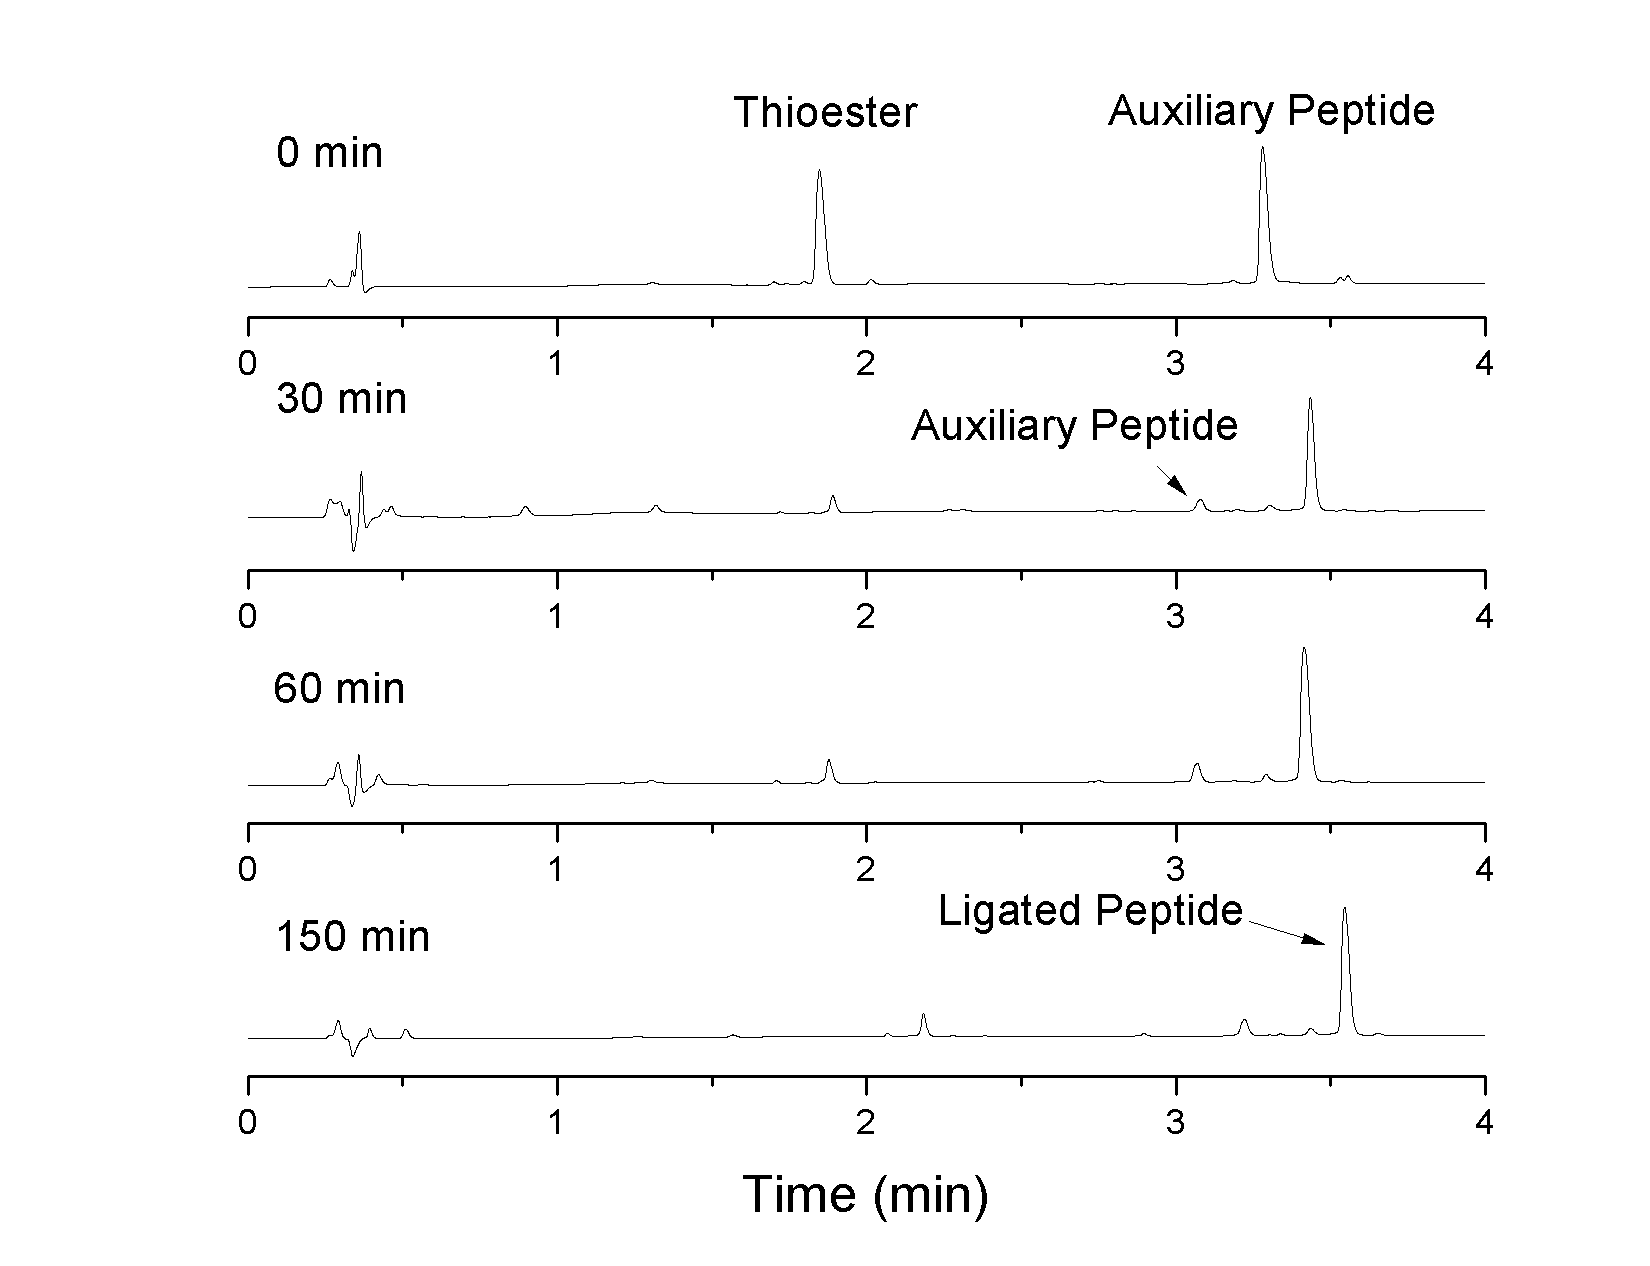
\includegraphics[max width=\textwidth]{brligation.png}
        \caption{UPLC of the time-course for the ligation of 4-bromophenyl auxiliary-peptide \cmpd+{cmpd:auxiliarypeptide.one}}
        \label{fig:brligation}
    \end{figure}

    \subsubsection{Ligation of Auxiliary Peptide \cmpd+{cmpd:auxiliarypeptide.two}}

    The ligation of auxiliary peptide \cmpd{cmpd:auxiliarypeptide.two} again occurred rapidly. The ligation was highly selective under the experimental conditions with complete conversion of \cmpd{cmpd:auxiliarypeptide.two} to the desired ligated peptide \cmpd{cmpd:auxiliarydipeptide.two}. The other peptide fragments in \ref{fig:meoligationtime} arise from the presence of excess thioester \cmpd{cmpd:thioester} post-ligation. The thiophenol aryl thioester \cmpd{cmpd:lyragthiophenol} is formed \insitu. The ligated auxiliary peptide \cmpd{cmpd:auxiliarydipeptide.two} can undergo a second thioester exchange in the presence of the \insitu generated thiophenol aryl thioester \cmpd{cmpd:lyragthiophenol} to form \cmpd{cmpd:dithioester}.

    \begin{figure}[!htpb]
        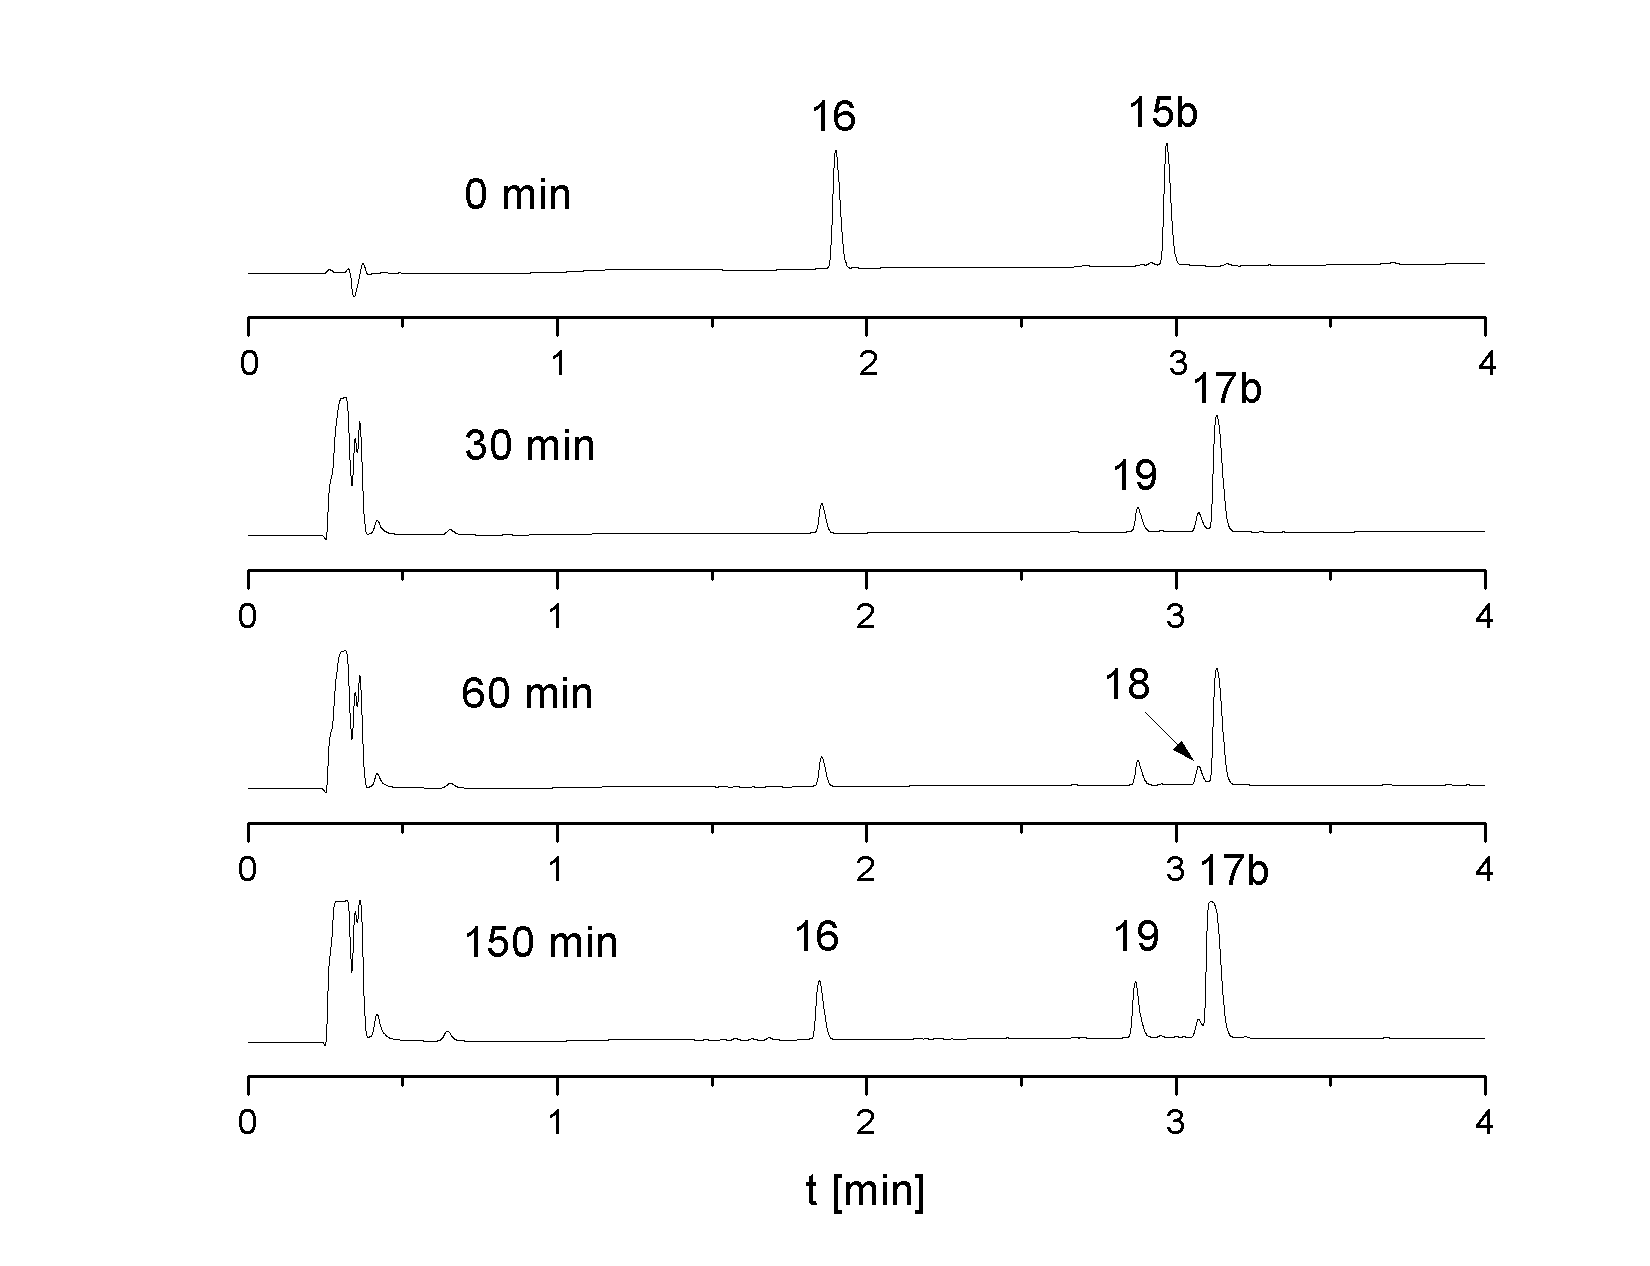
\includegraphics[max width=\textwidth]{meoligation.png}
        \caption{UPLC of the time-course for the ligation of 4-methoxyphenyl auxiliary-peptide \cmpd+{cmpd:auxiliarypeptide.two}}
        \label{fig:meoligationtime}
    \end{figure}

    Both ligation products were purified by preparative HPLC to yield the ligated auxiliary peptides \cmpd{cmpd:auxiliarydipeptide.one} (\SI{83}{\percent} yield) and \cmpd{cmpd:auxiliarydipeptide.two} (\SI{87}{\percent} yield) as white solids.

    \begin{figure}[!htpb]
        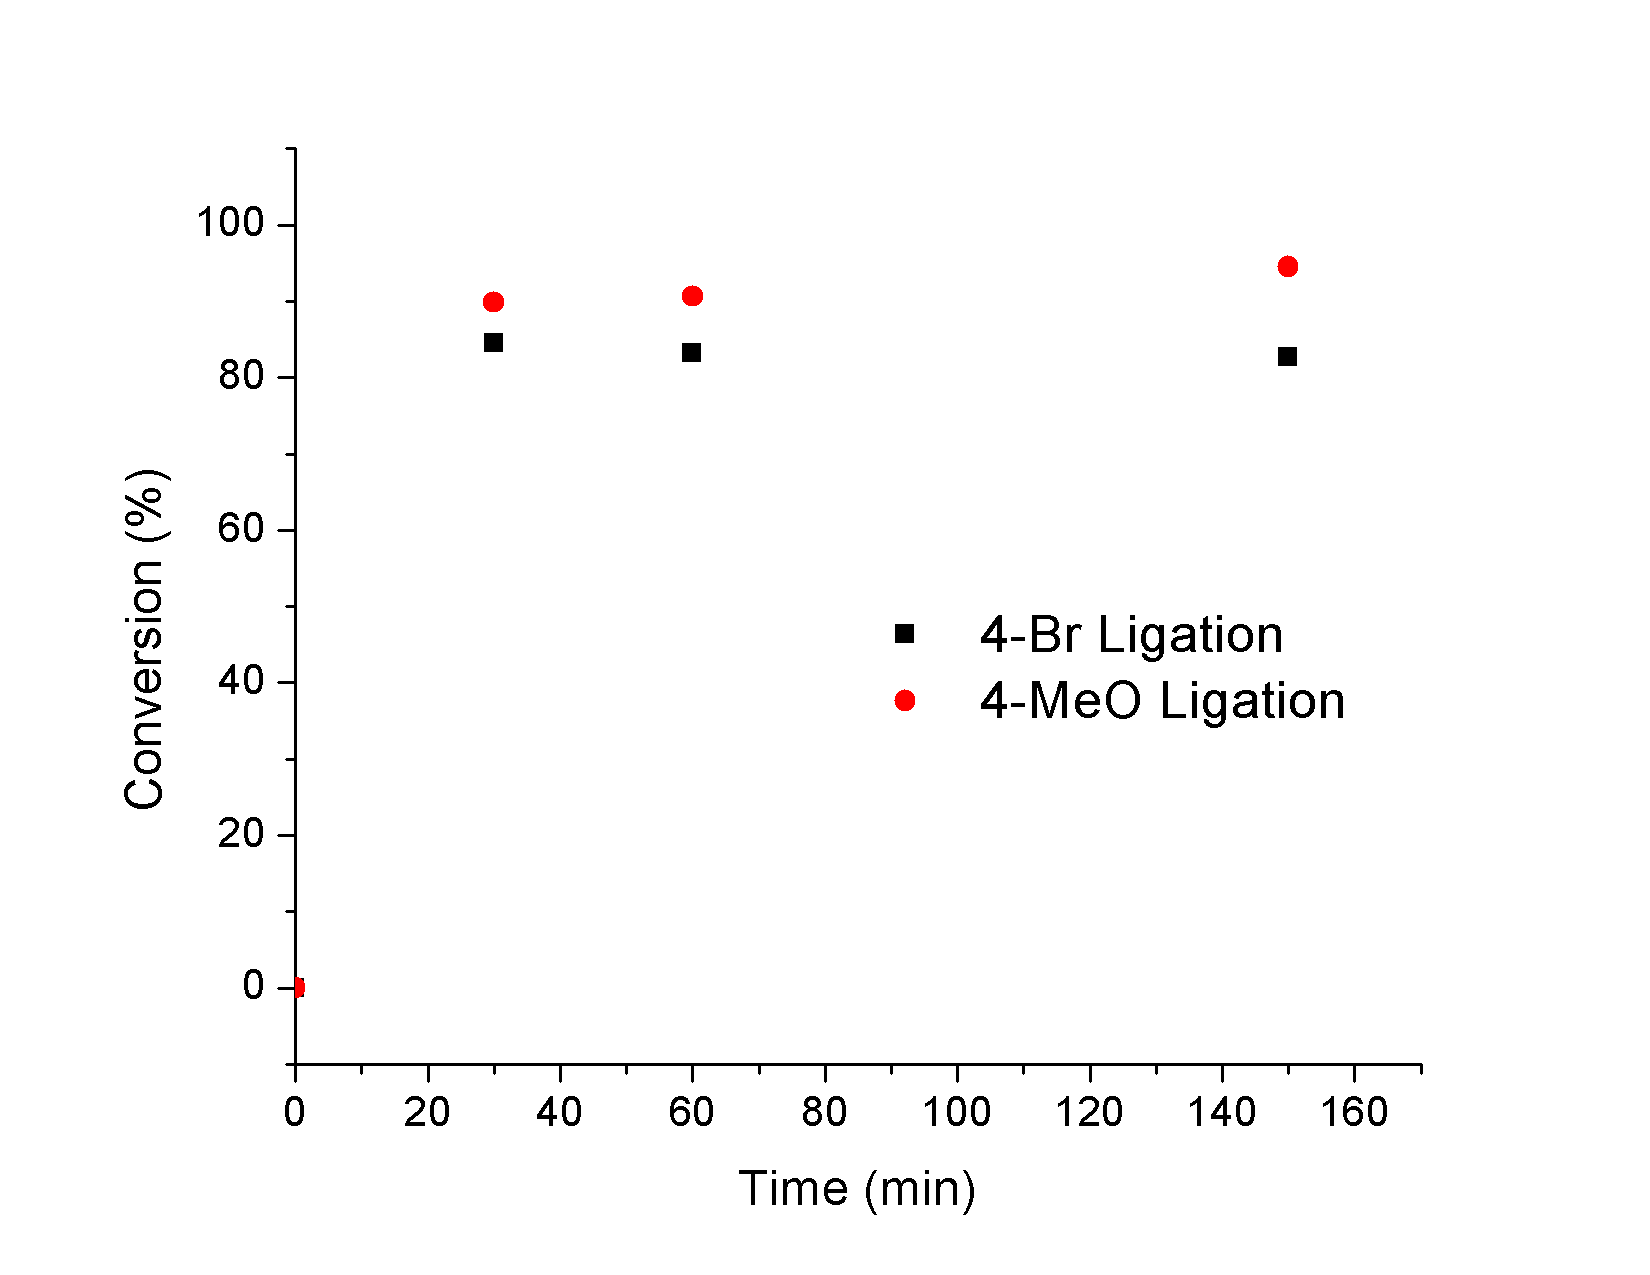
\includegraphics[max width=\textwidth]{combinedligation.png}
        \caption{Rate of ligation for both auxiliary peptides at the model Gly-Gly site.}
    \end{figure}

    It is clear that both auxiliaries can promote rapid, selective peptide ligation at a Gly-Gly junction. These results compare favorably to those obtained by Macmillan and Anderson with their acid labile auxiliary \cmpd{cmpd:trimethoxymercapto} at the same junction\cite{macmillan_rapid_2004}.

    Further trials at other more challenging ligation sites should be performed before significant comparisons  made between the ligation effectiveness of our two auxiliaries.

  \subsection{Auxiliary Cleavage}

    The ligation auxiliaries must be removable if they are to be synthetically useful for peptide synthesis. To begin, we subjected \cmpd{cmpd:auxiliarydipeptide.one} to the aqueous TCEP promoted cleavage conditions (100 mM TCEP, 400 mM morpholine, \SI{50}{\celsius}) previously examined in our group. We were pleasantly surprised to observe \SI{73}{\percent} conversion to the native peptide \cmpd{cmpd:dipeptide} (H-LYRAGGRAEYSGLG-\ch{NH2}) within \SI{24}{\hour}. This positive result was marred by the observation of the peptide backbone cleavage product \cmpd{cmpd:formylgraeysglg} (\IUPAC{N\|-formyl\|-GRAEYSGLG\|-\ch{NH2}}) as a side product (\ref{fig:br50cleave100}).

    In the hopes of minimizing peptide degradation we reexamined the cleavage of \cmpd{cmpd:auxiliarydipeptide.one} at room temperature with a lower TCEP concentration (20 mM). However these milder cleavage conditions lead to a large reduction in the rate of auxiliary removal. UPLC analysis indicated just \SI{26}{\percent} conversion after \SI{24}{\hour} (\ref{fig:brcleavage}).

    At this point, we reflected on Wan and Danishefsky's free radical based, TCEP promoted selective cysteine desulfurization \cite{wan_free-radical-based_2007}. With that work in mind, we hypothesised that the cleavage may be proceed proceeding via a rate limiting bimolecular TCEP promoted desulfurization step. A subsequent room temperature cleavage in the presence of 400 mM TCEP provided excellent results.  UPLC analysis indicated complete consumption of the ligated auxiliary peptide \cmpd{cmpd:auxiliarydipeptide.one} after \SI{4}{\hour}. The native peptide \cmpd{cmpd:dipeptide} was observed as the almost exclusive peptide product after \SI{24}{\hour} (\ref{fig:brrtcleavage}).

    Significantly a fragment of mass 282.19 Da was observed indicating the formation of the phosphoranyl species \IUPAC{3,3',3''-phosphorothionyltripropanoic acid} (M\textsubscript{calc}. 282.03 Da). These results suggest TCEP promoted desulfurization is a rate controlling step during the auxiliary cleavage.

    \begin{figure}[!htpb]
        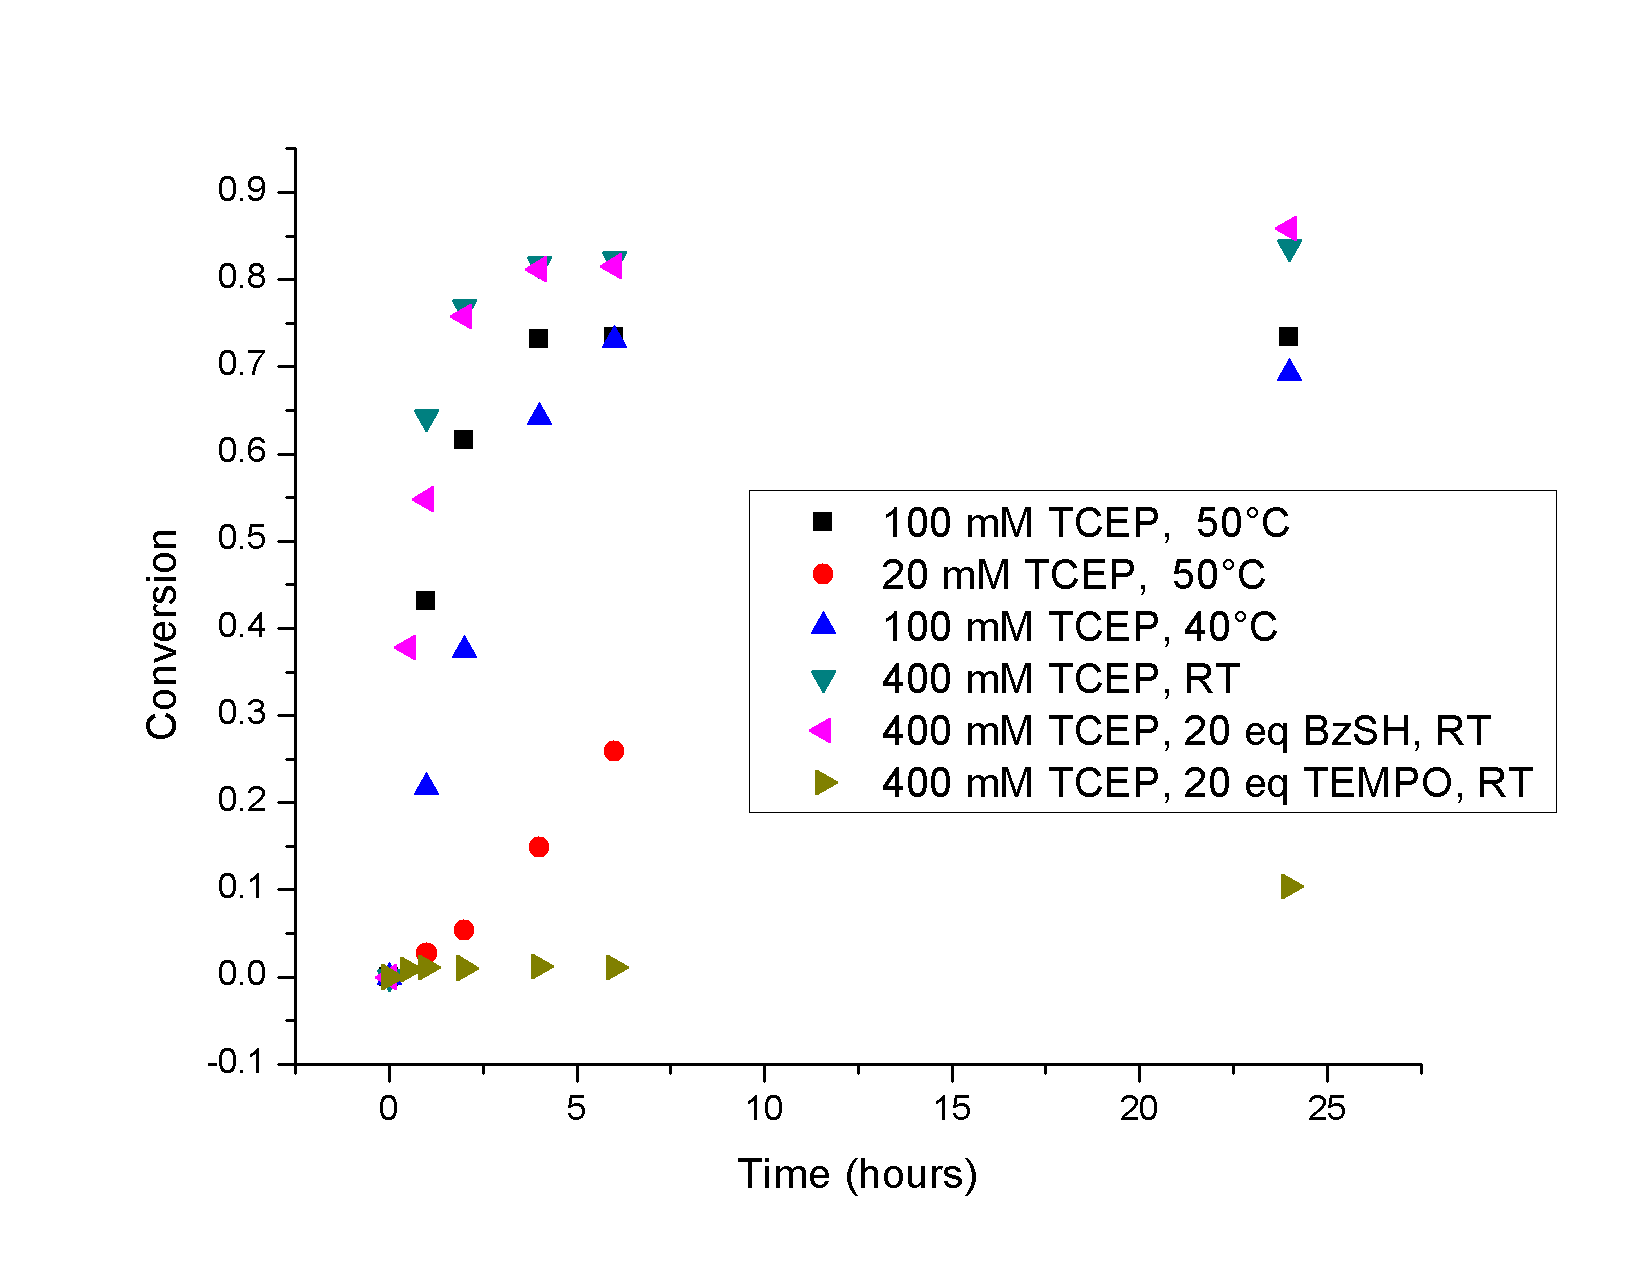
\includegraphics[max width=\textwidth]{brcombined.png}
        \caption{Influence of cleavage conditions on the rate of auxiliary \cmpd+{cmpd:auxiliarydipeptide.one} removal}
        \label{fig:brcleavage}
    \end{figure}

    It is notable that negligible product formation was observed when the stable free radical TEMPO (20 eq.) was added to the cleavage mixture (\ref{fig:brcleavage}). This result, while not conclusive, does further support our hypothesis that a radical process is in play.

    We proceeded to repeat a subset of these successful cleavage experiments on our second auxiliary-peptide \cmpd{cmpd:auxiliarydipeptide.two}. Again we observed rapid cleavage of our ligation auxiliary to provide the desired peptide \cmpd{cmpd:dipeptide}. The conversion was found to be somewhat higher with the (4-methoxyphenyl) bearing \cmpd{cmpd:auxiliarydipeptide.two} as shown in \ref{fig:brmeocleavage}.

    \begin{figure}[!htpb]
        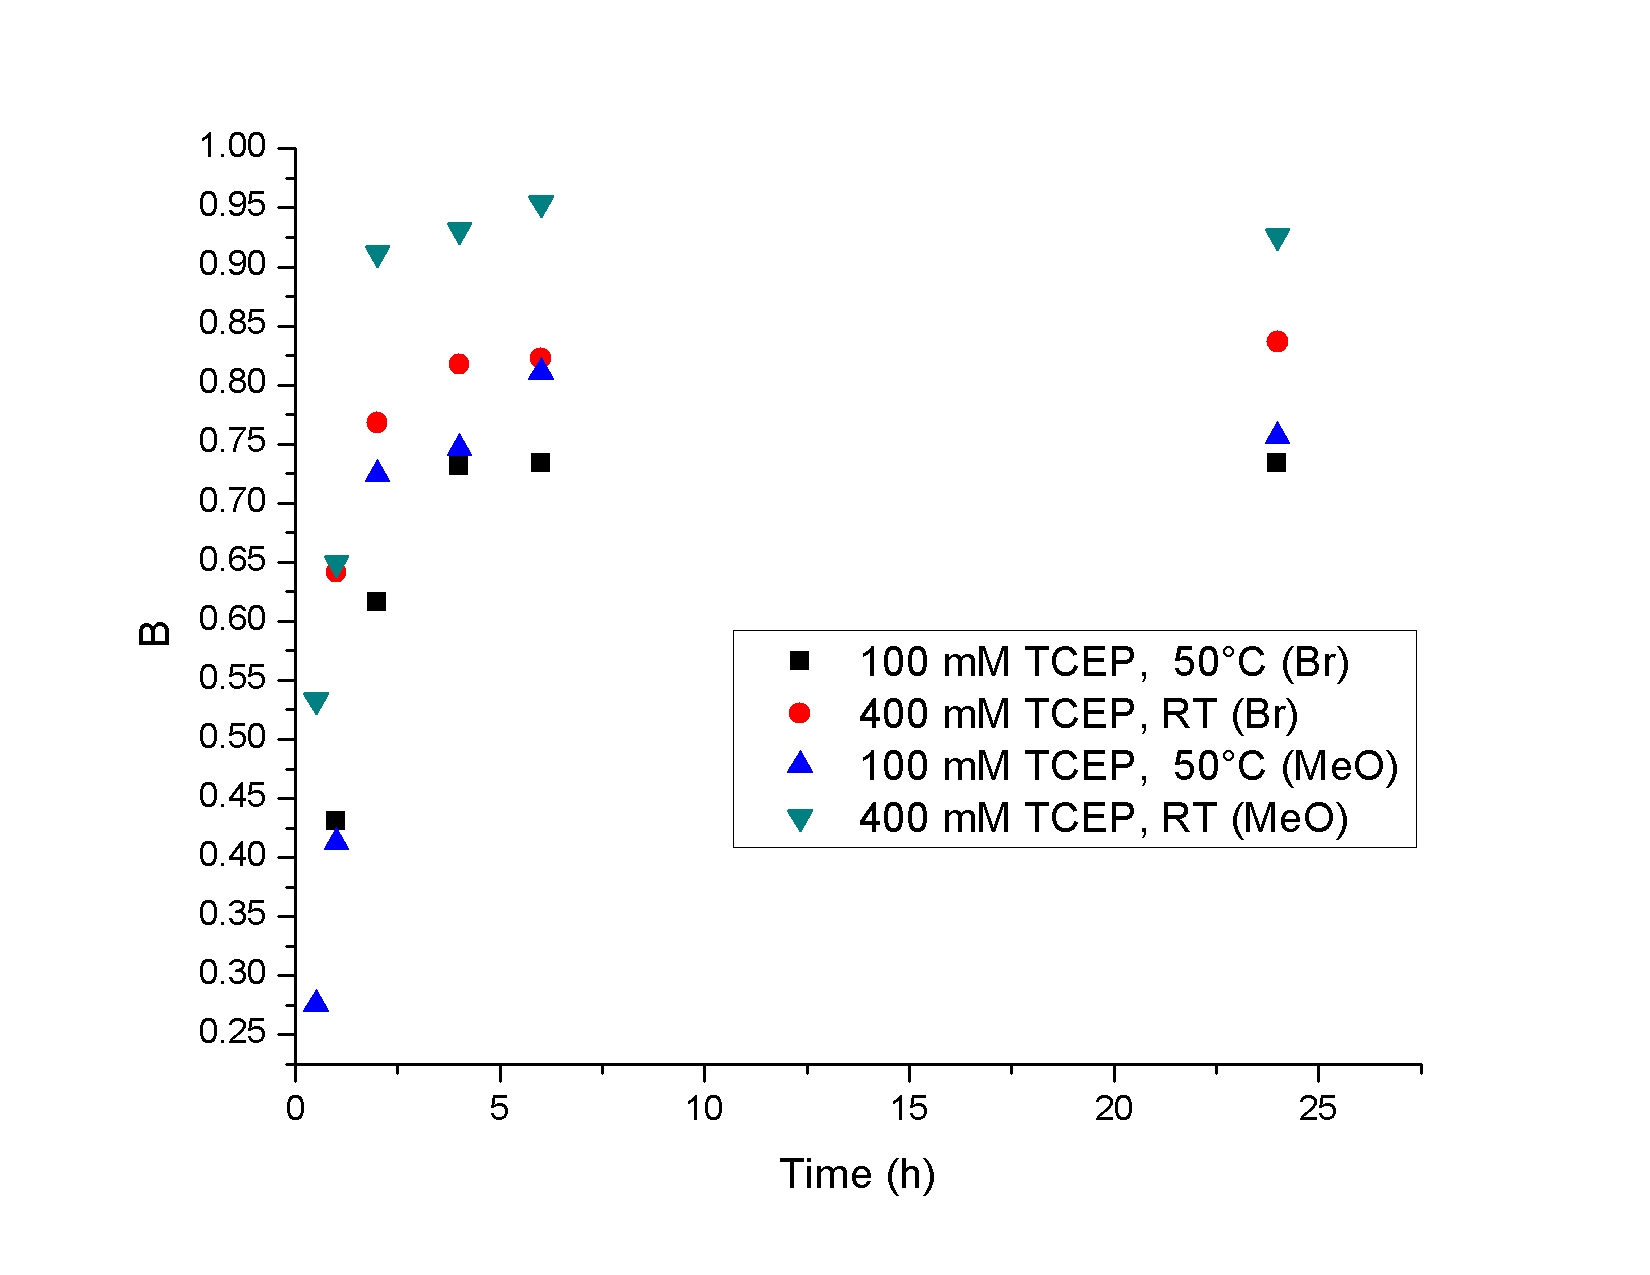
\includegraphics[max width=\textwidth]{brmeocombined.png}
        \caption{Comparison of the cleavage rate for both auxiliary peptides.}
        \label{fig:brmeocleavage}
    \end{figure}

    \cmpd{cmpd:auxiliarydipeptide.two} was subjected to the standard cleavage conditions (100 mM TCEP, \SI{50}{\celsius}) in the presence of the water-soluble radical initiator VA-044 (2eq. and 20 eq.). The radical initator producer a significant increased in the rate of cleavage (\ref{fig:meocleavagerate}). However the final yield of the native peptide was impacted by the extensive formation of an N-methylated peptide side product \cmpd{cmpd:nmethylpeptide} (up to \SI{35}{\percent}) and by desulfurisation of the auxiliary to give \cmpd{cmpd:meodesulfur} (\ref{fig:meoinitatorcleavage}).

    The radical initiator may be promoting the formation of a benzyl radical before intermolecular TCEP promoted desulfurization has had an opportunity to occurred.  Subsequent C-C bond scission would result in the formation of the observed N-methylated peptide product. We suspect that further work will allow the rates of intermolecular desulfurisation and radical formation to be matched. This may allow us to take advantage of the radical initator provided rate increases while minimising the production of unwanted peptide degradation side products.

    % \subsubsection{Post Cleavage Auxiliary Products
    % check the mass spec. Cursury search didn't indicated products. a radical polymerisbeation of the auxiliary cleavage fragments may be a possibility.
    %   in

% ------------------------------------------------------------------------


%%% Local Variables:
%%% mode: latex
%%% TeX-master: "../thesis"
%%% End:
